\documentclass{article}
\usepackage{nips07submit_e,times}
\usepackage{multirow}
\usepackage{graphics}
\usepackage{graphicx}


%\documentstyle[nips07submit_09,times]{article}


\title{Proposal:\\ME algorithm for Hierarchical Dirichilet Process and its Extensions}


\author{}



\newcommand{\fix}{\marginpar{FIX}}
\newcommand{\new}{\marginpar{NEW}}

\begin{document}
Donglai Wei and Erik Sudderth \\
Department of Computer Science\\
Brown University\\
Providence, RI 02912 \\
\texttt{\{donglai\_wei,sudderth\}@cs.brown.edu} \\

\makeanontitle

\begin{abstract}We here develop a  Maximize-Expectation(ME) learning algorithm for Hierarchical Dirichilet Process(HDP).
 We first show the advantage of ME algorithm to learn Dirichlet Process Mixture model with synthetic data. 
Then we use Chinese Restaurant Franchise(CRF) representation to construct ME algorithm for HDP. 
Later, we extend the ME algorithm to learn Hierarchical Pitman-Yor Process(HPY) model, which generalizes HDP with more flexiblility. 
Implementing our novel learning method, hopefully we will improve the learning performance of HPY model for shared segmentation problem.

\end{abstract}

\section{BackGround}
\subsection{Hierarchical Dirichilet Process}
During clustering, we may not only want to separate observations into different groups but also wish these groups to share common features. 
For example, in document modeling, the aim is to cluster words within the documents into different topics. 
When clustering documents from NIPS in machine learning and  computer vision, 
we may wish to allow topics like \textquotedblleft graphical model \textquotedblright and \textquotedblleft optimization\textquotedblright to be shared among them. 
\\ \\
Hierarchical Dirichilet Process(HDP), which natually handles the problem above, was formally introduced into unsupervised learning in Teh at.el[2].
Figure 1 shows the graphical model for DP mixture and HDP. But due to the complexity, the extant learning methods developed for HDP are far from maturity.
\subsection{ME Algorithm}
Consider a probabilistic model P(x,w,$\alpha$),where x is observed random variable, w hidden variable and $\alpha$ hyperparameter.   
Given a data set D, a typical task in machine learning is to maximize the likelihood function P(D $| \alpha$) by marginaling out hidden variable w. 
But the exact learining is often intractable. Variational Bayesian algorithms can give a reasonable lower bound for the likelihood by approximating the true distribution of hidden variables P (w $|$ D) based on Kullback-Leibler (KL) divergence. 
For our clustering problems, hidden variables are divided into two classes: cluster assignment variable z and model parameters $\theta$. 
Heuristically, we factorize the distribution P(w$|$D,$\alpha$)=P($\theta$, z$|$ D,$\alpha$) $\approx$ q (z)q ($\theta$) and update the estimated distribution for one hidden variable at a time. 
This results in the update: 
\begin{center}
$q (\theta ) \propto exp(E[log P(\thetaθ, z, D)]_{q(z)} ) \longleftrightarrow q (z) \propto  exp(E[log P(\theta, z, D)]_{q (\theta )})$.
\end{center}

This is the well-known Meanfield algorithm, which maintains a disribution over parameters (known as E-step).
Also, we can decide to estimate a maximum a posterior(MAP) value for the hidden variable (known as M-step). 
Discussed in [4], we can have four combinations of E-step and M-step for z and $\theta$. 
In this way, K-means belong to MM algorithm while Meanfield belongs to EE algorithm. 
But for most of the time, people may just want the optimal solution for the cluster assignment z instead of the real distribution of q(z).
Also, the cluster assignment variable z is discrete and high dimensional, which makes the update formula hard to compute. 
So instead of maintaining the huge matrix for q(z), we may just pick out the MAP estimator(M-step) for q(z).
Since we don't want to be too greedy to also take M-step for q($\theta$), we end up with ME algorithm.
In the next section, we are going to show the advantage of ME algorithm for learning DP mixture model.

  
\section{Preliminary Result}

We test Meanfield algorithm (EE) [1], Collapsed Meanfield algorithm(Collapsed EE)[5] and ME algorithm [3] implemented by Kurihara on the synthetic data, 200 random samples drawn from Gaussian of four mixtures.
We set almost same hyperparameters(except the one to generate mixture components) for these three algorithms and test with different initial cluster numbers.
Results are summarized in table 1. 
From figure 3 and 4, we can see that to some degree both EE and Collapsed EE suffer from local minimas and initialization.
Three variants of ME algorithms are tested here. Though the hierarchical clustering methods work perfect on this synthetic data, for real data top-down method uses heuristic criterion to split and merge while bottom-up method may have difficulty maintaining the huge distance matrix.
We here only try a naive local search. Though it does not perform well enough at first glance, it can be improved with advanced search algorithms and it fits best into Chinese Restaurant Franchise representation for Constructing HDP.
\begin{figure}[h] 
  \begin{minipage}[b]{0.5\textwidth} 
    \centering 
    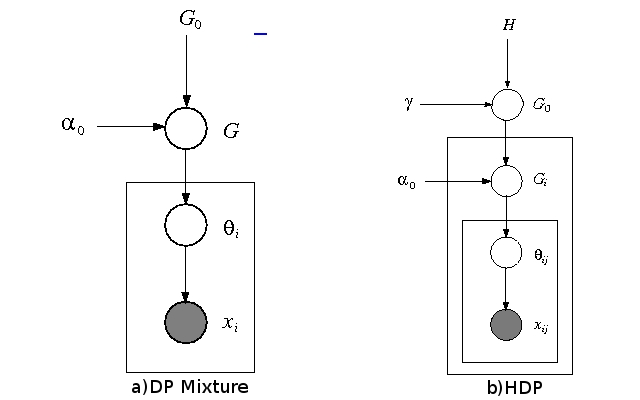
\includegraphics[width=0.8\textwidth]{dp.jpg} 
    \caption{Graphical Model for DP mixture and HDP} 
    \label{fig:by:table} 
  \end{minipage}% 
  \begin{minipage}[b]{0.5\textwidth} 
    \centering 
    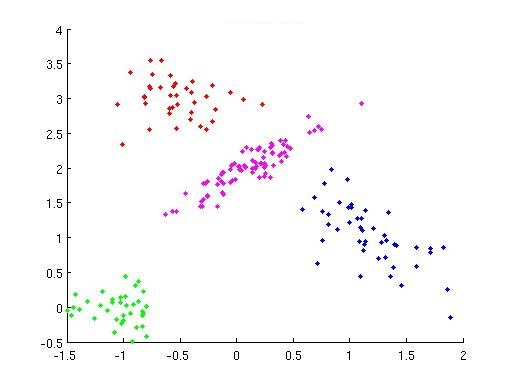
\includegraphics[width=0.8\textwidth]{truth.jpg} 
    \caption{Ground Truth 200 data from Gaussian Mixture} 
    \label{fig:by:table}  
   \end{minipage}% 
   \end{figure}
\begin{figure}[h] 
  \begin{minipage}[b]{0.5\textwidth} 
    \centering 
    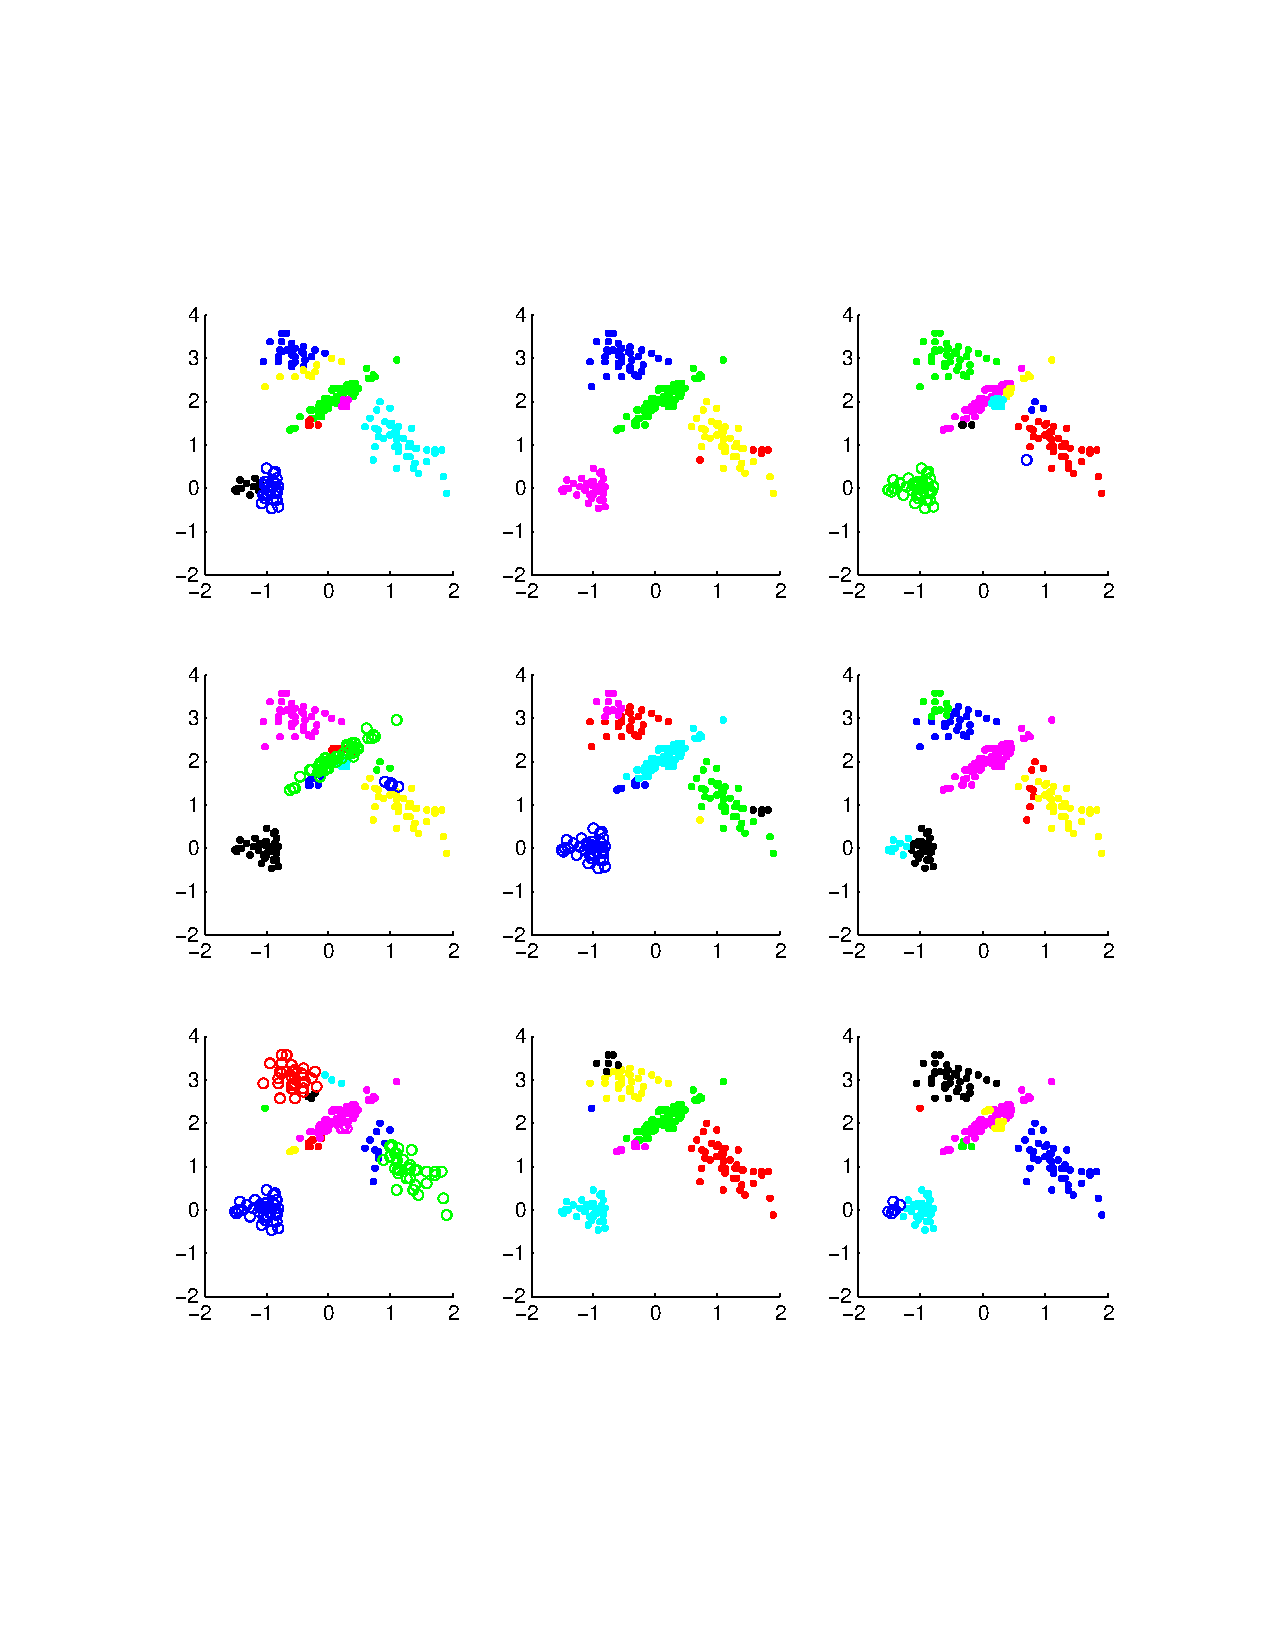
\includegraphics[width=0.8\textwidth]{BJ.pdf} 
    \caption{EE with random initialization, 20 inital clusters} 
    \label{fig:by:table} 
  \end{minipage}% 
  \begin{minipage}[b]{0.5\textwidth} 
    \centering 
    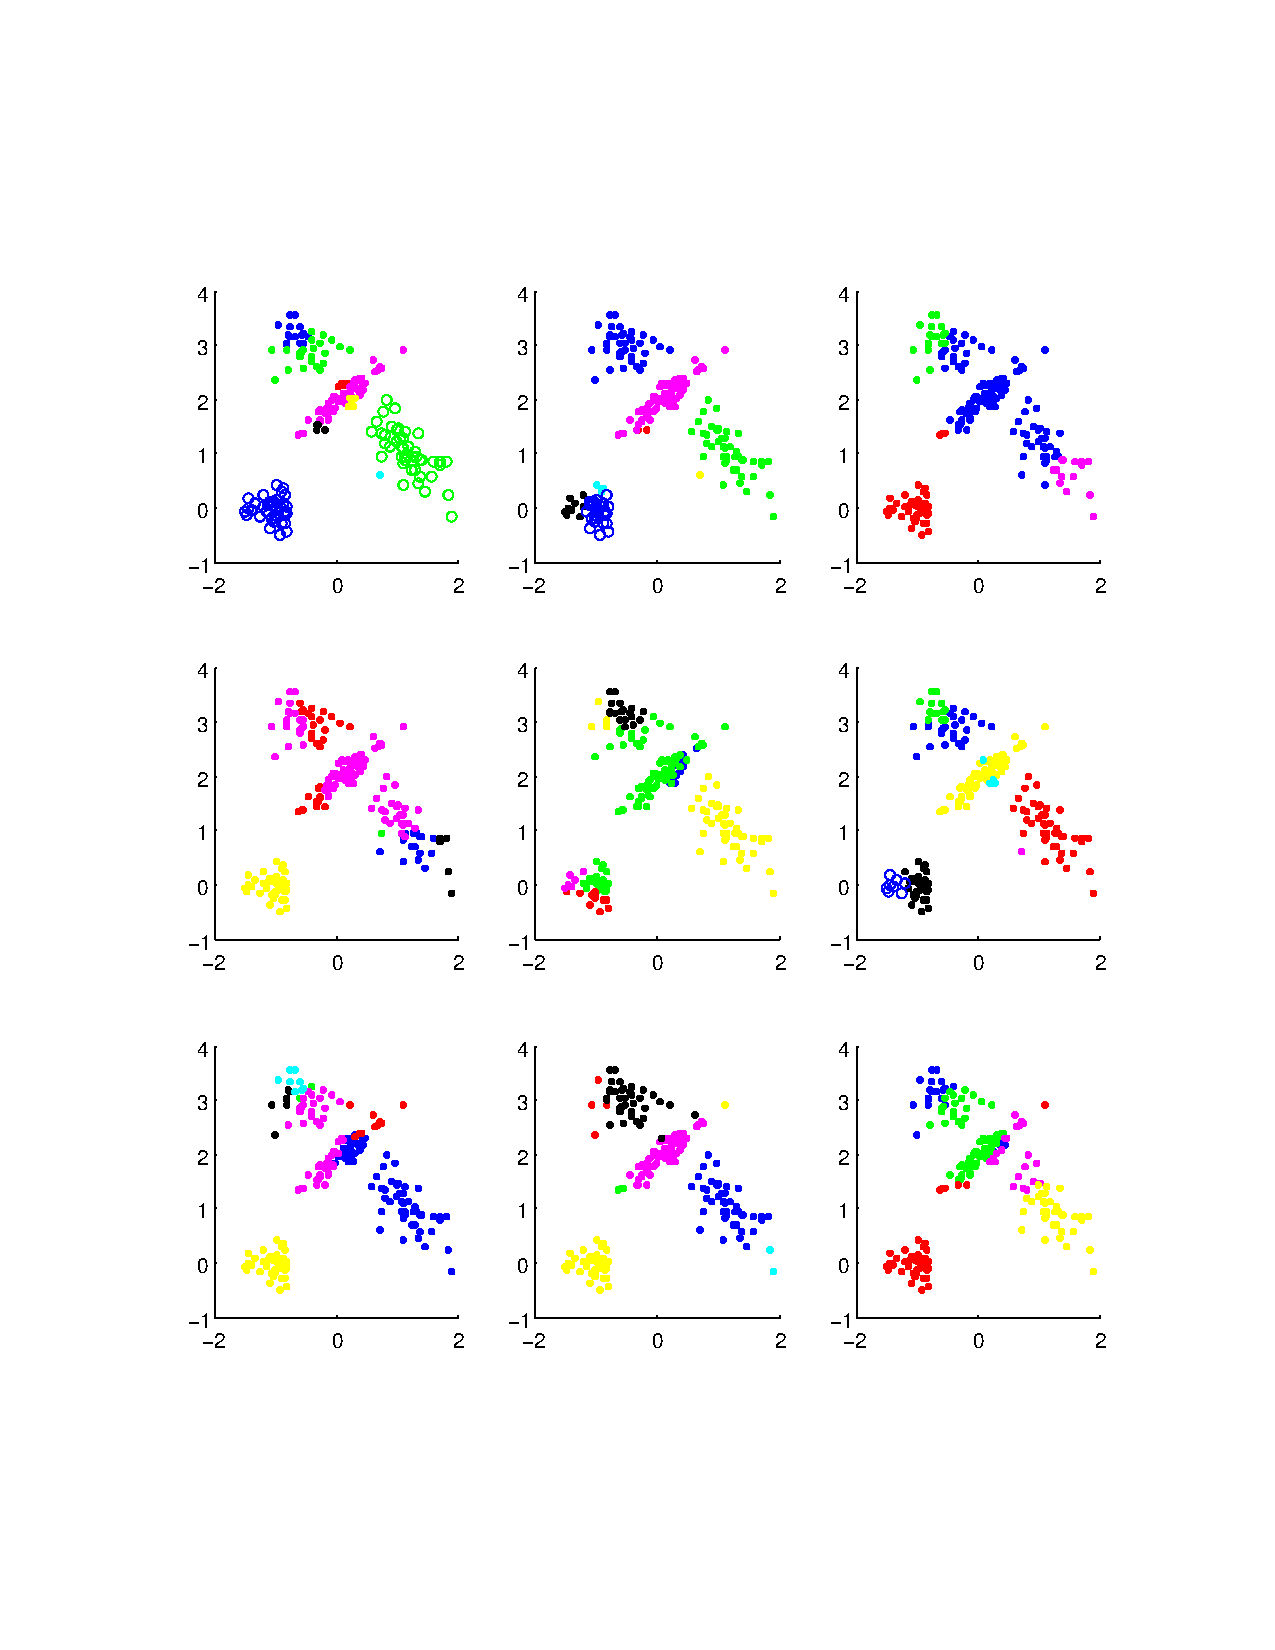
\includegraphics[width=0.8\textwidth]{cdb.pdf} 
    \caption{Collapsed EE with random initialization, 20 inital clusters}
    \label{fig:by:table}  
   \end{minipage}% 
   \end{figure}
\begin{table}[t]
\caption{Comparison of EE, Collapsed-EE and ME algorithms for DP mixture(with mean and std)}
\begin{center}
\begin{tabular}{|l|l|l|l|}
\hline
{\bf Learning Algorithm} &{\bf Initial Cluster Numbers} &{\bf Number of clusters}  &{\bf RandIndex} \\ 
\hline 
\multirow{2}{*}{EE(sampled initialization)} & 10 & 4.1(0.3) & 0.99(0.00) \\
					    & 20 & 4.1(0.3) & 0.99(0.00)\\
\hline
\multirow{2}{*}{EE(random initialization)}  & 10 & 6.9(1.2)&  0.97(0.01) \\
					    & 20 & 7.6(1.7)&  0.93(0.02) \\
\hline
\multirow{2}{*}{Collapsed EE}               & 10 & 5.6(1.6)&  0.90(0.22) \\
					    & 20 & 7.4(0.9)&  0.87(0.09) \\
\hline
\multirow{4}{*}{ME}                         & 1(Top-down) &    4  &  1 \\
					    & 200(Bottom-up) & 4  &  1 \\
					    & 200(Local search) & 15.5(3.9)&  0.83(0.09) \\
					    & 200(Local search+Merge) & 6.5(0.9)&  0.93(0.09) \\
\hline
\end{tabular}
\end{center}
\end{table}

\section{Research Plan}

-- 3.1:\ \ \ \ \textbf{Survey} the literature on \textbf{DP mixture} and \textbf{HDP} \\
-- 3.25: \textbf{Test} ME, EE, Collapsed EE algorithms for \textbf{DP Mixture} on a synthetic data set.\\
-- 4.15: \textbf{Develop} ME algorithm for \textbf{HDP} \\
-- 4.25: \textbf{Test} ME algorithm against Collapsed EE and Gibbs sampling for \textbf{HDP} model\\
-- 5.1: \ \ \textbf{Test} ME algorithm for learning \textbf{HPY} model for shared segmentation problems.\\
-- 5.10: \textbf{Write} documentation and technical report\\

\section{References}
\small{
[1]  Blei,D,M, Jordan,M.I, and Ng, A. Y. (2003), “Hierarchical Bayesian Models for Applications 
  in Information Retrieval,” in Bayesian Statistics, vol. 7, pp. 25–44 

[2] Ghahramani, Z., \& Beal, M. J. (2000). Variational inference for Bayesian mixtures of                                                          ̈
  factor analysers. In S. A. Solla, T. K. Leen, \& K.-R. Muller (Eds.), Advances in neural
  information processing systems, 12. Cambridge, MA: MIT Press.

[3] K. Kurihara and M. Welling. Bayesian K-means as a
 ”maximization-expectation” algorithm. Neural Computation, 2008

[4] Y. W. Teh, M. I. Jordan, M. J. Beal, and D. M. Blei. Hierarchical Dirichlet processes. Journal of the 
American Statistical Association, 101(476):1566–1581, 2006.

[5] Y. W. Teh, K. Kurihara and M. Welling. Collapsed Variational Inference for HDP
NIPS 2007

}


\end{document}
